\chapter{Methodology} % Main chapter title

\label{ch:meth}

\lhead{Chapter 2. \emph{Methodology}}

\section{Solution Outline}
We have devised a systematic approach involving key steps to optimise our testing process. Initially, a robust deployment method ensures the swift installation of software onto designated testing devices, establishing the foundation for a streamlined testing procedure. Next, an intuitive interface facilitates smooth, bidirectional data exchange within the wireless testing network. This interface is a crucial communication link between the testing environment and the software under evaluation.
Following deployment, our process involves meticulously executing a comprehensive test framework. This framework rigorously evaluates collected data, systematically examining the performance and functionality of the software. The subsequent data analysis phase culminates in generating a detailed bug report, a valuable resource for our development team.

\section{Architechture}
\subsection{Hardware architecture}
The basic hardware architecture of the wBMS involves multiple gateways and nodes. The nodes contain the sensors of the system and relay the information to the gateways who in turn, communicate with the host application to ultimately provide the collected information to the end user.
To provide the firmware to the embedded devices, we flash the devices with J-Link debuggers \cite{jlink}. We then create the network between the various devices in the system with the help of software
\begin{figure}[ht]
    \centering
    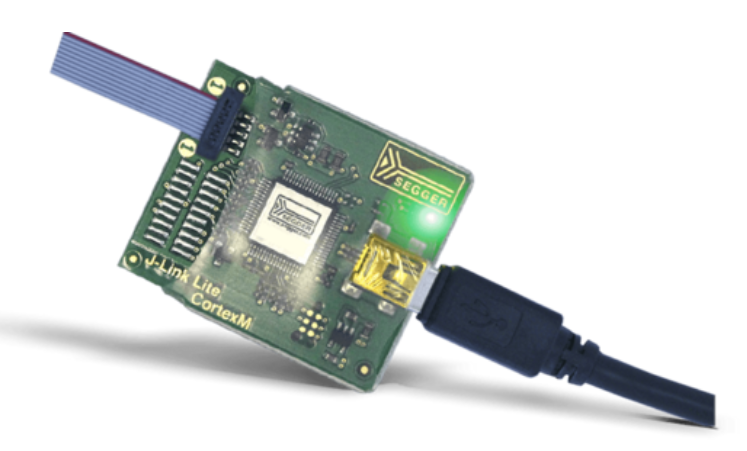
\includegraphics[scale=0.5]{../Figures/jlink.png}
    \caption{J-Link lite debugger}
    \label{fig:jlink}
\end{figure}

\subsection{Software architecture}
\subsubsection{System software architecture}
The system software architecture is mainly present to control the network between the gateways and the nodes.
This involves a GUI application with specific exposed API endpoints which will enable communication of the network with any test framework built.
This will eventually allow us to automate certain tests instead of manually performing them from the GUI.
\subsubsection{Testing software architecture}
To make the test framework easy to access and maintain, python \cite{pythondocs} was decided to be used to create the test framework.
The initial design of this framework was done with a hybrid approach involving both scripting and Object Oriented Programming concepts.
To improve this design, another framework was designed with Pytest \cite{pytest} solely using Object Oriented concepts.
\section{Workflow}
\subsection{Testing ideologies}
To design test cases that exhaustively cover all possible scenarios, we must adhere to certain aspects of the Software Test Life Cycle (STLC). This mainly consists of 4 steps:
\begin{enumerate}
    \item Test planning
    \item Test case development
    \item Test environment setup
    \item Test execution
\end{enumerate}

\subsubsection{Test planning}
During the initial step, the software testing team meticulously crafts essential testing strategies, making it the focal point of the process.
This critical phase, marked by significance, involves formulating a comprehensive plan to guide the testing process.
Typically, the responsibility for establishing project costs and required efforts rests with the team lead or manager \cite{ref32}.
This planning phase commences upon the conclusion of the requirement collection stage, signifying a pivotal transition in the testing lifecycle.
The paramount outcome of this preparatory phase is the crystallization of a finalized test plan and strategy.
This meticulously designed framework is the guiding document, dictating the subsequent testing procedures and ensuring adherence to the established protocols.

\subsubsection{Test case development}
After outlining a strategy for the tests, the team proceeds to gather the necessary data for implementation.
The team then organizes the gathered data to align with various test cases, ensuring comprehensive coverage of all possible scenarios.
After completing the design for individual test cases, each case is linked in a chain within the Responsibility Traceability Matrix \cite{ref33}.
This matrix serves as a structured framework, mapping the relationship between test cases and their associated responsibilities.

\subsubsection{Test environment setup}
The development team or the client actively undertakes a standalone task to determine the environment for software evaluation.
Simultaneously, the testing team, taking an active role, formulates specific unit test cases to ensure the environment's readiness.

\subsubsection{Text execution}
In this phase, the testing team initiates the execution of test cases based on the decided strategy and environment.
If certain tests fail, the team reports the specific defect to the development team using a bug-tracking system.
Ideally, every failed test case should be linked to at least one problem, aiding in the identification of issues with the software \cite{ref34}
In the case of a test case being blocked by a design flaw, it is appropriately marked.<br>
Subsequently, a comprehensive report, encompassing all failed and blocked test cases, is prepared and provided to the development team for further action.

\subsection{Test execution with the framework}
As part of the test execution, we have chosen to work with pytest because of its simplicity and support.
This is a widely used library and hence will also be easy for future managers to oversee any bugs within the code itself.

This library also provides support with common development environments such as VSCode to allow running tests without having to use multiple terminals to achieve the end goal.
\begin{figure}[ht]
    \centering
    \begin{minipage}{0.45\textwidth}
        \centering
        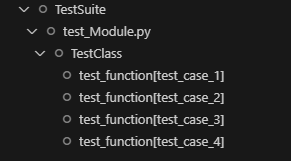
\includegraphics{../Figures/untested.png}
        \caption{Untested test cases as collected by pytest on VSCode}
    \end{minipage}\hfill
    \begin{minipage}{0.45\textwidth}
        \centering
        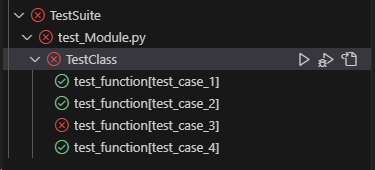
\includegraphics[scale=0.9]{../Figures/tested.png}
        \caption{After testing on VSCode}
    \end{minipage}
\end{figure}

Pytest also allows us to use various plugins like pytest-html \cite{pytest-html} that will allow us to automatically generate HTML and XML reports.
These can be used by other teams to create consolidated reports if needed.
\begin{figure}[ht]
    \centering
    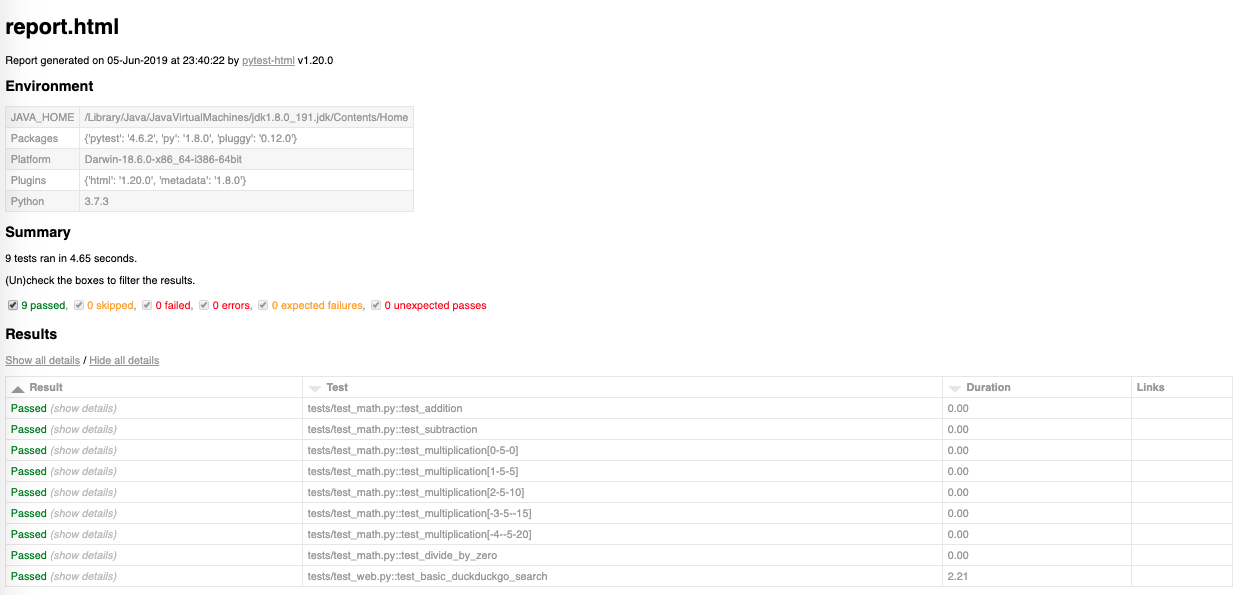
\includegraphics[scale=0.6]{../Figures/pytesthtml.png}
    \caption{Sample pytest HTML report \cite{htmlreport}}
\end{figure}
\newpage
\section{Automation of the workflow}
The test framework has only solved a part of our problem to automate testing of the firmware.
In order to achieve complete automation, we can use CI/CD pipeline software like Jenkins \cite{jenkins} to trigger the test framework to build based on new releases.
This will allow us to generate test reports very quickly after each release. This will allow the development team to patch any issues with the firmware and will eventually ensure that the end user of the system will not have to experience buggy software.
